\documentclass[aspectratio=169,10pt]{beamer}

% ── Theme & colors ──────────────────────────────────────────────
\usetheme{Madrid}
\usecolortheme{seahorse}
\definecolor{csblue}{RGB}{0,75,135}
\setbeamercolor{structure}{fg=csblue}
\setbeamercolor{title}{fg=white,bg=csblue}
\setbeamercolor{frametitle}{fg=white,bg=csblue}
\setbeamertemplate{navigation symbols}{}
\setbeamertemplate{footline}{%
  \leavevmode\hbox{%
    \begin{beamercolorbox}[wd=.33\paperwidth,ht=2.5ex,dp=1ex,center]{author in head/foot}%
      \usebeamerfont{author in head/foot}\insertshortauthor
    \end{beamercolorbox}%
    \begin{beamercolorbox}[wd=.34\paperwidth,ht=2.5ex,dp=1ex,center]{title in head/foot}%
      \usebeamerfont{title in head/foot}\insertshorttitle
    \end{beamercolorbox}%
    \begin{beamercolorbox}[wd=.33\paperwidth,ht=2.5ex,dp=1ex,right]{date in head/foot}%
      \usebeamerfont{date in head/foot}\insertframenumber/\inserttotalframenumber\hspace*{2ex}
    \end{beamercolorbox}}%
}

% ── Packages ────────────────────────────────────────────────────
\usepackage[utf8]{inputenc}
\usepackage[T1]{fontenc}
\usepackage{amsmath,amssymb}
\usepackage{booktabs}
\usepackage{graphicx}
\usepackage{tikz}
\usetikzlibrary{shapes.geometric,arrows.meta,positioning,fit,calc}
\usepackage{algorithm}
\usepackage{algpseudocode}
\usepackage{multirow}
\usepackage{xcolor}
\usepackage{hyperref}

% ── Metadata ────────────────────────────────────────────────────
\title[Domain-Specific LLM for Reliability]{Developing a Domain-Specific LLM through\\Self-Instruct for Reliability Engineering}
\author[Dalban \& Drouilhet]{Alexandre Dalban \and Elora Drouilhet}
\institute[CentraleSup\'elec]{%
  Laboratoire G\'enie Industriel (LGI)\\
  CentraleSup\'elec -- Universit\'e Paris-Saclay}
\date{April 2026}

% ════════════════════════════════════════════════════════════════
\begin{document}

% ── Slide 1: Title ──────────────────────────────────────────────
\begin{frame}
\titlepage
\vspace{-1em}
\begin{center}
  \small\textbf{Supervisors:} Dr.\ Zhiguo Zeng, Jean Meunier-Pion\\[4pt]
  \footnotesize\texttt{alexandre.dalban@student-cs.fr} \quad\texttt{elora.drouilhet@student-cs.fr}\\[2pt]
  \footnotesize Code \& data: \url{https://github.com/ADnocap/Reliability-Domain-Specific-LLM}
\end{center}
\end{frame}

% ── Slide 2: Outline ───────────────────────────────────────────
\begin{frame}{Outline}
\tableofcontents
\end{frame}

% ════════════════════════════════════════════════════════════════
\section{Motivation}
% ── Slide 3: Motivation ────────────────────────────────────────
\begin{frame}{Why Reliability Engineering Needs Specialized LLMs}
\begin{columns}[T]
\column{0.55\textwidth}
\textbf{The problem:}
\begin{itemize}
  \item General-purpose LLMs (GPT-4, Claude) struggle with \textbf{precise numerical computation} in reliability engineering
  \item Best frontier models achieve only $\sim$50--80\% on hand-written reliability problems
  \item \textbf{No existing dataset or benchmark} for this domain
\end{itemize}

\vspace{0.5em}
\textbf{Why it matters:}
\begin{itemize}
  \item Reliability engineering underpins safety-critical industries (aerospace, nuclear, medical devices)
  \item Computations involve Weibull/exponential distributions, MTTF, system reliability, Bayesian inference
\end{itemize}

\column{0.4\textwidth}
\centering
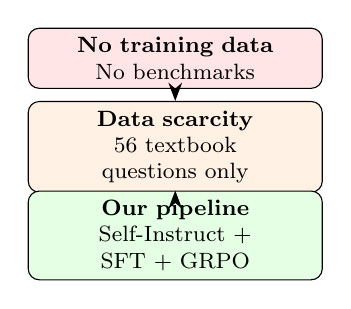
\begin{tikzpicture}[scale=0.75, every node/.style={font=\footnotesize}]
  \node[draw, rounded corners, fill=red!10, text width=3.5cm, align=center] (prob) at (0,3) {\textbf{No training data}\\No benchmarks};
  \node[draw, rounded corners, fill=orange!10, text width=3.5cm, align=center] (challenge) at (0,1.5) {\textbf{Data scarcity}\\56 textbook questions only};
  \node[draw, rounded corners, fill=green!10, text width=3.5cm, align=center] (sol) at (0,0) {\textbf{Our pipeline}\\Self-Instruct + SFT + GRPO};
  \draw[-{Stealth}, thick] (prob) -- (challenge);
  \draw[-{Stealth}, thick] (challenge) -- (sol);
\end{tikzpicture}
\end{columns}
\end{frame}

% ── Slide 4: Bootstrapping Challenge ──────────────────────────
\begin{frame}{The Bootstrapping Challenge}
\begin{block}{Central question}
  How to build a high-quality training dataset from only \textbf{56 seed questions}?
\end{block}

\vspace{0.5em}
\textbf{Key challenges:}
\begin{itemize}
  \item Manually creating reliability engineering Q\&A pairs is \textbf{prohibitively expensive} --- each problem requires expert knowledge
  \item Self-Instruct [Wang et al.\ 2023] can bootstrap data, but \textbf{same-model consistency checks} are trivially satisfied in technical domains (92--97\% pass rate)
  \item Generating harder questions yields \textbf{diminishing returns} (+65 hard questions $\to$ only +2.0\%)
  \item Prior SFT attempts on small data ($\leq$51 samples) caused \textbf{catastrophic forgetting} ($-8.19$pp)
\end{itemize}

\vspace{0.5em}
\textbf{Our approach:}
\begin{enumerate}
  \item \textbf{Cross-model verification:} Claude generates, GPT-5.4 independently verifies
  \item \textbf{Paraphrase augmentation} (inspired by MetaMath): scale data through surface diversity
  \item \textbf{SFT then GRPO:} supervised learning for structure, RL to explore reasoning
\end{enumerate}
\end{frame}

% ════════════════════════════════════════════════════════════════
\section{Research Problem}
% ── Slide 5: Research Questions ────────────────────────────────
\begin{frame}{Research Problem}
\begin{alertblock}{Central question}
  How can we adapt a general-purpose LLM to reliability engineering\\
  using only \textbf{56 seed questions}, without catastrophic forgetting?
\end{alertblock}

\vspace{0.5em}
\textbf{Sub-problems:}
\begin{enumerate}
  \item \textbf{Data scarcity:} How to bootstrap a high-quality training set from 56 textbook questions?
  \item \textbf{Quality control:} How to ensure synthetic questions are correct and non-trivial?
  \item \textbf{Catastrophic forgetting:} How to gain domain accuracy without losing generalization?
  \item \textbf{RL on small data:} Can GRPO work with only $\sim$266 training questions?
\end{enumerate}
\end{frame}

% ════════════════════════════════════════════════════════════════
\section{State of the Art}
% ── Slide 6: Related Work ──────────────────────────────────────
\begin{frame}{State of the Art}
\begin{columns}[T]
\column{0.48\textwidth}
\textbf{Self-Instruct \& Synthetic Data}
\begin{itemize}
  \item Self-Instruct [Wang et al.\ 2023]: bootstrap data from seeds
  \item WizardLM, Alpaca: scaling instruction data
  \item \textcolor{red}{Limitation: same-model consistency $\to$ trivially satisfied}
  \item SearchInstruct [Li et al.\ 2025]: external grounding
\end{itemize}

\vspace{0.5em}
\textbf{Data Augmentation for Reasoning}
\begin{itemize}
  \item MetaMath [Yu et al.\ 2024]: rephrasing $>$ difficulty
  \item PersonaMath: persona-driven variants
  \item Model collapse risk [Shumailov et al.\ 2024]
\end{itemize}

\column{0.48\textwidth}
\textbf{RL for Reasoning}
\begin{itemize}
  \item RLHF / DPO: preference-based alignment
  \item \textbf{GRPO} [Shao et al.\ 2024]: group-relative advantages, no critic needed
  \item DeepSeek-R1: scaled GRPO for reasoning
  \item DAPO [Yu et al.\ 2025]: dynamic sampling for small datasets
\end{itemize}

\vspace{0.5em}
\textbf{Domain Adaptation}
\begin{itemize}
  \item MedPaLM, ChatLaw, Code Llama
  \item QLoRA + NEFTune for parameter efficiency
  \item \textcolor{red}{No prior work on reliability engineering}
\end{itemize}
\end{columns}
\end{frame}

% ════════════════════════════════════════════════════════════════
\section{Methodology}
% ── Slide 7: Pipeline Overview ─────────────────────────────────
\begin{frame}{Methodology Overview: 5-Stage Pipeline}
\centering
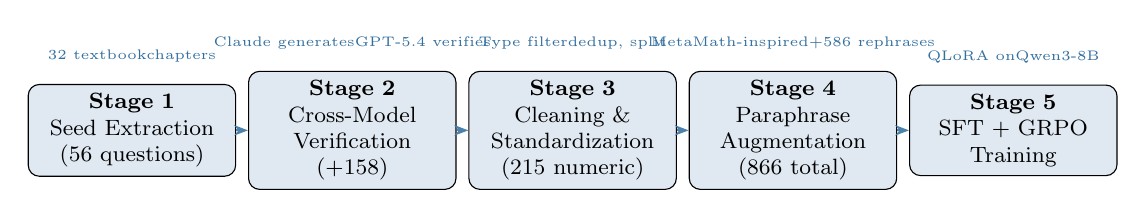
\begin{tikzpicture}[
  node distance=0.4cm and 0.15cm,
  stage/.style={draw, rounded corners, fill=csblue!12, minimum height=1cm, text width=2.4cm, align=center, font=\footnotesize},
  arr/.style={-{Stealth[length=5pt]}, thick, csblue!70},
  lbl/.style={font=\tiny, text=csblue!80}
]
  \node[stage] (s1) {\textbf{Stage 1}\\Seed Extraction\\(56 questions)};
  \node[stage, right=of s1] (s2) {\textbf{Stage 2}\\Cross-Model\\Verification\\(+158)};
  \node[stage, right=of s2] (s3) {\textbf{Stage 3}\\Cleaning \&\\Standardization\\(215 numeric)};
  \node[stage, right=of s3] (s4) {\textbf{Stage 4}\\Paraphrase\\Augmentation\\(866 total)};
  \node[stage, right=of s4] (s5) {\textbf{Stage 5}\\SFT + GRPO\\Training};

  \draw[arr] (s1) -- (s2);
  \draw[arr] (s2) -- (s3);
  \draw[arr] (s3) -- (s4);
  \draw[arr] (s4) -- (s5);

  \node[lbl, above=0.15cm of s1] {32 textbook\\chapters};
  \node[lbl, above=0.15cm of s2] {Claude generates\\GPT-5.4 verifies};
  \node[lbl, above=0.15cm of s3] {Type filter\\dedup, split};
  \node[lbl, above=0.15cm of s4] {MetaMath-inspired\\+586 rephrases};
  \node[lbl, above=0.15cm of s5] {QLoRA on\\Qwen3-8B};
\end{tikzpicture}

\vspace{0.8em}
\begin{columns}[T]
\column{0.45\textwidth}
\textbf{Key innovation -- Cross-model verification:}
\begin{itemize}\small
  \item Claude Opus 4 generates questions
  \item GPT-5.4 independently solves them
  \item Keep only if answers match ($\leq 5\%$ tolerance)
\end{itemize}
\column{0.45\textwidth}
\textbf{Key innovation -- Paraphrase augmentation:}
\begin{itemize}\small
  \item Surface-level rephrases preserving math
  \item Verified by second model
  \item 586 paraphrases $\to$ \textbf{+18.6\%} accuracy
\end{itemize}
\end{columns}
\end{frame}

% ── Slide 8: SFT Setup & Hyperparameters ──────────────────────
\begin{frame}{Supervised Fine-Tuning: Setup \& Hyperparameters}
\begin{columns}[T]
\column{0.48\textwidth}
\textbf{Model selection:}
\begin{itemize}\small
  \item \textbf{Qwen3-8B} selected over Llama 3.1 8B
  \item Zero-shot baseline: 70.7\% vs 37.5\%
  \item Llama fine-tuning caused regression ($-1.4$pp on numeric)
  \item 4-bit quantization via QLoRA / Unsloth
\end{itemize}

\vspace{0.3em}
\textbf{Thinking mode insight:}
\begin{itemize}\small
  \item Qwen3 uses \texttt{<think>} blocks as scratch work
  \item Training data = polished solutions (no backtracking)
  \item Mismatch $\to$ overfitting to shallow pattern-matching
  \item \textbf{Solution:} disable thinking during SFT
\end{itemize}

\column{0.48\textwidth}
\textbf{Hyperparameters (26 experiments):}
\vspace{0.3em}

\centering
\begin{tabular}{@{}ll@{}}
  \toprule
  \textbf{Parameter} & \textbf{Value} \\
  \midrule
  LoRA rank / alpha & $r\!=\!16$, $\alpha\!=\!32$ \\
  LoRA targets & All attn + MLP layers \\
  Learning rate & $2\!\times\!10^{-4}$ (cosine) \\
  Optimizer & AdamW 8-bit \\
  Batch size & 2 (eff.\ 8 w/ grad accum) \\
  Max epochs & 8 (ES $\to$ epoch 4) \\
  NEFTune $\alpha$ & 5 \\
  Precision & BF16 \\
  Max seq.\ length & 2048 tokens \\
  \bottomrule
\end{tabular}

\vspace{0.4em}
\small\textbf{Evaluation:} greedy decoding, 10-fold CV,\\Wilcoxon signed-rank test
\end{columns}
\end{frame}

% ── Slide 9: SFT Results ─────────────────────────────────────
\begin{frame}{Supervised Fine-Tuning: Results \& Ablations}
\begin{columns}[T]
\column{0.48\textwidth}
\textbf{Results by dataset size:}
\vspace{0.3em}

\centering
\begin{tabular}{@{}lcccc@{}}
  \toprule
  \textbf{Dataset} & $N$ & Base & FT & $p$ \\
  \midrule
  v1 (cleaned) & 215 & 70.7 & 73.0 & 0.50 \\
  v2 (+hard)   & 280 & 71.0 & 73.0 & 0.69 \\
  v3 (+para.)  & 501 & 59.1 & 65.3 & 0.063 \\
  \textbf{v4 (+para.)} & \textbf{866} & \textbf{63.6} & \textbf{82.2} & \textbf{0.002} \\
  \bottomrule
\end{tabular}

\vspace{0.5em}
\textbf{Question flip ratio:}
\begin{itemize}\small
  \item 215 samples: 1.3:1 (23 gains vs 18 losses)
  \item \textbf{866 samples: 4.6:1} (206 gains vs 45 losses)
\end{itemize}

\column{0.48\textwidth}
\textbf{Key ablations (on 215 questions):}
\vspace{0.3em}

\centering
\begin{tabular}{@{}lcc@{}}
  \toprule
  \textbf{Variation} & $\Delta$ & $p$ \\
  \midrule
  \textbf{Best config} & \textbf{+2.3} & 0.50 \\
  Lower LR ($10^{-4}$) & $-0.5$ & 1.0 \\
  Higher NEFTune ($\alpha\!=\!7$) & $-1.3$ & 0.38 \\
  LoRA $r\!=\!8$ & $+1.4$ & 0.88 \\
  DPO (instead of SFT) & $-1.7$ & 0.63 \\
  \bottomrule
\end{tabular}

\vspace{0.5em}
\textcolor{csblue}{\textbf{Key findings:}}
\begin{itemize}\small
  \item Paraphrase augmentation $\gg$ hard questions\\(+18.6\% vs +2.0\%)
  \item DPO \textbf{hurts} on small datasets
  \item Threshold effect around 500 examples
\end{itemize}
\end{columns}
\end{frame}

% ── Slide 10: GRPO Algorithm ──────────────────────────────────
\begin{frame}{GRPO: Algorithm \& Reward Design}
\begin{columns}[T]
\column{0.52\textwidth}
\begin{block}{Group Relative Policy Optimization}
\begin{algorithmic}[1]\small
  \For{each question $q$}
    \State Sample $G\!=\!4$ completions $\{o_1, \ldots, o_G\}$ from $\pi_\theta$
    \State Score each with graded reward $r(o_i, q)$
    \If{$\sigma(\{r_i\}) = 0$} \textbf{skip} (DAPO filtering)
    \EndIf
    \State Normalize: $\hat{A}_i = \frac{r_i - \bar{r}}{\sigma_r + \varepsilon}$
    \State Update: $\mathcal{L} = -\frac{1}{G}\sum_i \hat{A}_i \cdot \frac{\log \pi_\theta(o_i|q)}{|o_i|}$
  \EndFor
\end{algorithmic}
\end{block}

\vspace{0.3em}
\textbf{Advantages over PPO / DPO:}
\begin{itemize}\small
  \item No critic model needed (group-relative baseline)
  \item No pre-computed preference pairs
  \item Verifiable numerical rewards --- no learned reward model
\end{itemize}

\column{0.44\textwidth}
\textbf{Graded reward function:}
\vspace{0.3em}

\centering
\begin{tabular}{@{}lc@{}}
  \toprule
  \textbf{Condition} & \textbf{$r(o,q)$} \\
  \midrule
  Error $\leq 0.1\%$ & $+1.0$ \\
  Error $\leq 1\%$ & $+0.8$ \\
  Error $\leq 5\%$ & $+0.4$ \\
  Error $> 5\%$ & $+0.01$ \\
  No boxed found & $0.0$ \\
  $>2$ boxed values (hedging) & $-0.3$ \\
  \bottomrule
\end{tabular}

\vspace{0.5em}
\small Graded structure provides \textbf{smooth reward landscape}: partially correct answers get positive signal, encouraging refinement rather than abandonment.

\vspace{0.3em}
Anti-hedging penalty discourages\\outputting multiple candidate answers.
\end{columns}
\end{frame}

% ── Slide 11: GRPO Data Split & Dynamic Sampling ─────────────
\begin{frame}{GRPO: Data split \& dynamic sampling (DAPO)}
\begin{columns}[T]
\column{0.48\textwidth}
\textbf{Training data split via base-model screening:}
\vspace{0.3em}

Each question evaluated \textbf{4 times} with base Qwen3-8B:

\vspace{0.3em}
\centering
\resizebox{\linewidth}{!}{ % <--- Ajout ici
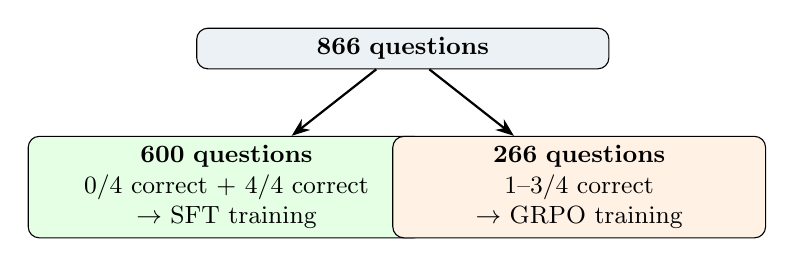
\begin{tikzpicture}[scale=0.8, every node/.style={font=\small}]
  \node[draw, rounded corners, fill=csblue!8, text width=5cm, align=center] (all) at (0,3) {\textbf{866 questions}};
  \node[draw, rounded corners, fill=green!10, text width=4.8cm, align=center] (sft) at (-2.8,0.8) {\textbf{600 questions}\\0/4 correct\ + 4/4 correct \\$\to$ SFT training};
  \node[draw, rounded corners, fill=orange!10, text width=4.5cm, align=center] (mixed) at (2.8,0.8) {\textbf{266 questions}\\1--3/4 correct\\$\to$ GRPO training};
  \draw[-{Stealth}, thick] (all) -- (sft);
  \draw[-{Stealth}, thick] (all) -- (mixed);
\end{tikzpicture}
} % <--- Et ici

\vspace{0.3em}
\small \textbf{Why this split?} 0/4 and 4/4 produce \textbf{zero reward variance} in GRPO (all generations same outcome) $\to$ no gradient signal. But they work fine for SFT. Only 1--3/4 questions have the natural variance GRPO needs.

\column{0.48\textwidth}
\textbf{Dynamic sampling (DAPO):}

\vspace{0.3em}
\begin{itemize}\small
  \item If all 4 generations produce the \textbf{same reward} $\to$ prompt is \textbf{discarded} (zero gradient signal)
  \item All correct (too easy) or all wrong (no positive signal)
  \item \textbf{Waste rate} = diagnostic metric:
  \begin{itemize}\footnotesize
    \item Rising $\to$ model is converging
    \item Initially high $\to$ poor data calibration
  \end{itemize}
\end{itemize}

\vspace{0.3em}
\textbf{GRPO hyperparameters:}
\vspace{0.2em}

\centering
\begin{tabular}{@{}ll@{}}
  \toprule
  \textbf{Parameter} & \textbf{Value} \\
  \midrule
  Generations per prompt & $G = 4$ \\
  Useful steps & 200 \\
  Learning rate & $1\!\times\!10^{-5}$ (cosine) \\
  KL coefficient ($\beta$) & 0 \\
  LoRA rank / alpha & $r\!=\!32$, $\alpha\!=\!32$ \\
  Max completion & 3072 tokens \\
  Temperature & 1.0 \\
  \bottomrule
\end{tabular}
\end{columns}
\end{frame}

% ════════════════════════════════════════════════════════════════
\section{Results}
% ── Slide 12: GRPO Results ────────────────────────────────────
\begin{frame}{GRPO results \& ablations}
\begin{columns}[T]
\column{0.52\textwidth}
\textbf{On 266 mixed-difficulty questions:}
\vspace{0.3em}

\centering
\begin{tabular}{@{}lcc@{}}
  \toprule
  \textbf{Model} & \textbf{Acc.} & $\Delta$ \\
  \midrule
  Base Qwen3-8B         & 50.4\% & --- \\
  SFT                   & 50.8\% & ref \\
  \midrule
  GRPO from scratch (step 80)    & 50.8\% & +0.4 \\
  \textbf{GRPO from SFT (step 80)} & \textbf{57.9\%} & \textbf{+7.5} \\
  GRPO from SFT (step 100) & 54.1\% & +3.7 \\
  GRPO from SFT (step 200) & 52.3\% & +1.9 \\
  \bottomrule
\end{tabular}

\vspace{0.5em}
\textbf{SFT warm-start ablation:}
\vspace{0.2em}

\centering
\begin{tabular}{@{}lccc@{}}
  \toprule
  \textbf{Init} & \textbf{Acc.} & $\Delta$ & \textbf{Waste} \\
  \midrule
  Fresh LoRA & 50.8\% & +0.4 vs base & 29.3\% \\
  \textbf{SFT} & \textbf{57.9\%} & \textbf{+7.5 vs base} & 23.1\% \\
  \bottomrule
\end{tabular}

\column{0.44\textwidth}
\textbf{Overfitting dynamics:}
\vspace{0.3em}

\centering

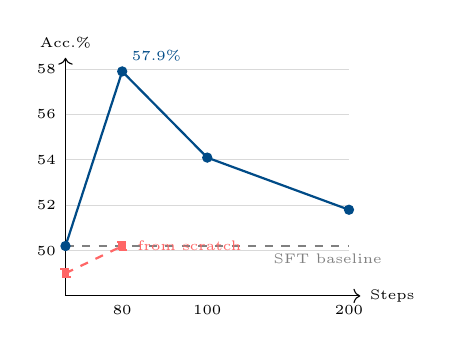
\begin{tikzpicture}[scale=0.72]
  \draw[->] (0,0) -- (5.2,0) node[right] {\tiny Steps};
  \draw[->] (0,0) -- (0,4.2) node[above] {\tiny Acc.\%};
  \foreach \y/\l in {0.8/50,1.6/52,2.4/54,3.2/56,4.0/58} {
    \draw[gray!30] (0,\y) -- (5,\y);
    \node[left,font=\tiny] at (0,\y) {\l};
  }
  \foreach \x/\l in {1/80,2.5/100,5/200} {
    \node[below,font=\tiny] at (\x,0) {\l};
  }
  \draw[dashed, gray] (0,0.88) -- (5,0.88);
  \node[right,font=\tiny,gray] at (3.5,0.65) {SFT baseline};
  \draw[thick, csblue, mark=*] plot coordinates {(0,0.88) (1,3.96) (2.5,2.44) (5,1.52)};
  \node[above right,font=\tiny,csblue] at (1,3.96) {57.9\%};
  \draw[thick, red!60, dashed, mark=square*] plot coordinates {(0,0.4) (1,0.88)};
  \node[right,font=\tiny,red!60] at (1.1,0.88) {from scratch};
\end{tikzpicture}

\vspace{0.3em}
\small
\textbf{Findings:}
\begin{itemize}\footnotesize
  \item Peak at step 80, then degradation
  \item 266 questions insufficient for sustained RL
  \item SFT init: lower waste rate (23\% vs 29\%)\\$\to$ more efficient learning
  \item GRPO from scratch: \textbf{no improvement}
\end{itemize}
\end{columns}
\end{frame}

% ── Slide 13: Holdout & Frontier ──────────────────────────────
\begin{frame}{Generalization \& comparison with frontier models}
    
    \textbf{54-question independent holdout:}
    \vspace{0.5em}

    % Tableau étalé sur toute la largeur
    \centering
    \begin{tabular*}{\textwidth}{@{\extracolsep{\fill}}lccccc@{}}
        \toprule
        \textbf{Model} & \textbf{Acc.} & $\Delta$ & W$\to$R & R$\to$W & $p$ \\
        \midrule
        Base Qwen3-8B & 53.7\% & --- & --- & --- & --- \\
        SFT & \textcolor{red}{\textbf{33.3\%}} & \textcolor{red}{$-20.4$} & 4 & 15 & \textbf{0.019} \\
        GRPO from scratch & 55.6\% & $+1.9$ & 3 & 2 & 1.000 \\
        GRPO from SFT & 50.0\% & $-3.7$ & 9 & 7 & 0.803 \\
        \bottomrule
    \end{tabular*}

    \vspace{1em}

    \begin{alertblock}{The SFT Paradox}
        SFT \textbf{degrades} generalization ($-20.4$pp, $p=0.019$) yet is \textbf{essential} as GRPO initialization: $+7.5$pp in-distribution from SFT vs $+0.4$pp from scratch.

        \vspace{0.3em}
        \small Neither GRPO variant significantly changes holdout performance (both $p > 0.8$).
    \end{alertblock}

    \vspace{0.5em}
    \textbf{Hypothesis:} SFT teaches domain format/vocabulary; GRPO optimizes reasoning on that foundation.

    \vfill % Pousse la note en bas de page
    {\footnotesize\color{gray} \textit{Note: 54 questions ($\approx$1.85pp each) --- insufficient to reliably detect small improvements or regressions. Results should be interpreted as directional.}}

\end{frame}

% ── Slide: Frontier Model Comparison ───────────────────────────
\begin{frame}{Comparison with Frontier Models}
\begin{columns}[T]
\column{0.55\textwidth}

\centering
\begin{tabular}{@{}lcc@{}}
  \toprule
  \textbf{Model} & \textbf{v4 (500q)} & \textbf{Holdout (54q)} \\
  \midrule
  Claude Sonnet 4.6      & 92.4\% & 81.1\% \\
  o3-mini                & 86.4\% & 77.1\% \\
  Gemini 3.1 Pro         & 76.4\% & 82.6\%$^\dagger$ \\
  \midrule
  Qwen3-8B (base)        & 63.6\%$^*$ & 53.7\% \\
  Qwen3-8B (SFT)         & 82.2\%$^*$ & 33.3\% \\
  Qwen3-8B (SFT+GRPO)   & \textit{pending} & 50.0\% \\
  \bottomrule
\end{tabular}

\vspace{0.3em}
{\scriptsize $^*$10-fold CV. $^\dagger$23/54 extracted.}

\column{0.43\textwidth}
\textbf{Key takeaways:}
\begin{itemize}\small
  \item Our SFT model (82.2\%) places \textbf{between o3-mini and Gemini 3.1 Pro}
  \item Despite being \textbf{$\sim$100$\times$ smaller} (8B vs.\ frontier)
  \item SFT accuracy measured via 10-fold CV (not directly comparable but informative)
  \item Gap to Claude Sonnet 4.6 (92.4\%) remains substantial
\end{itemize}

\vspace{0.5em}
{\footnotesize\color{gray} \textit{Note: holdout = 54 questions only. Results are directional, not statistically significant comparisons.}}
\end{columns}
\end{frame}

% ════════════════════════════════════════════════════════════════
\section{Advantages \& Limitations}
% ── Slide 14: Advantages & Limitations ─────────────────────────
\begin{frame}{Advantages and Limitations}
\begin{columns}[T]
\column{0.48\textwidth}
\textbf{\textcolor{green!50!black}{Advantages:}}
\begin{itemize}\small
  \item \textbf{Data-efficient:} 56 seeds $\to$ 866 verified examples
  \item \textbf{Statistically rigorous:} 10-fold CV, Wilcoxon test ($p=0.002$)
  \item \textbf{Cross-model verification:} higher quality than self-consistency
  \item \textbf{Paraphrase $\gg$ difficulty:} +18.6\% vs +2.0\%
  \item \textbf{8B model competitive with frontier} on domain tasks (see previous slide)
  \item \textbf{Self-instruct ceiling effect} identified: novel finding for synthetic data
  \item \textbf{Reproducible:} open-source code and data
\end{itemize}

\column{0.48\textwidth}
\textbf{\textcolor{red}{Limitations:}}
\begin{itemize}\small
  \item \textbf{Single numeric answer only:} all Q\&A require exactly one numerical answer --- excludes derivations, proofs, conceptual questions, and multi-part problems
  \item \textbf{Narrow seed base:} all 866 examples derived from only 56 seed questions --- models may specialize on a subset of reliability concepts
    \item \textbf{Small holdout set:} 54 questions, limits statistical power for OOD conclusions
  \item \textbf{Self-instruct ceiling:} synthetic data stays within the generator's capability envelope (Claude & ChatGPT)
  \item \textbf{GRPO gains modest:} $+7.5$pp in-distribution (vs base), no significant effect on holdout
  \item \textbf{Single domain:} not yet validated on other engineering fields
\end{itemize}
\end{columns}
\end{frame}

% ════════════════════════════════════════════════════════════════
\section{Conclusion \& Perspectives}
% ── Slide 15: Conclusion ──────────────────────────────────────
\begin{frame}{Conclusion and Perspectives}
\begin{columns}[T]
\column{0.48\textwidth}
\textbf{Key contributions:}
\begin{enumerate}\small
  \item \textbf{Data augmentation pipeline:} 56 textbook seeds $\to$ 866 verified examples via cross-model generation and paraphrase augmentation
  \item \textbf{Adapted self-instruct} with cross-model verification (replaces same-model consistency)
  \item \textbf{Self-instruct ceiling effect} identified: generators stay within their capability envelope
  \item \textbf{SFT pipeline:} 8B model competitive with frontier models on reliability engineering
  \item \textbf{GRPO exploration:} +7.5pp in-distribution, no significant holdout degradation, but limited by data scale
\end{enumerate}

\column{0.48\textwidth}
\textbf{Future work:}
\begin{enumerate}\small
  \item Broader domain coverage: reliability engineering spans many sub-fields (Bayesian, Markov, fault trees, \ldots) $\to$ need more diverse seed data beyond 56 questions to cover the full scope
  \item Introduce KL penalty ($\beta > 0$) to reduce GRPO overfitting
  \item Early stopping on holdout validation rather than training loss
  \item Ground data generation in textbook source material (SearchInstruct approach)
  \item Extend to formula derivation and other engineering domains
\end{enumerate}
\end{columns}
\end{frame}

% ════════════════════════════════════════════════════════════════
\section{Work Organization}
% ── Slide 16: Work Organization ───────────────────────────────
\begin{frame}{Work Organization}
\textbf{Duration:} October 2025 -- April 2026 ($\sim$6 months, $\sim$250 combined hours)

\vspace{0.5em}
\centering
\begin{tabular}{p{5.5cm}cc}
  \toprule
  \textbf{Task} & \textbf{Alexandre} & \textbf{Elora} \\
  \midrule
  Seed extraction \& data pipeline       & \textbullet\textbullet\textbullet & \textbullet \\
  Cross-model verification               & \textbullet\textbullet\textbullet & \textbullet \\
  Paraphrase augmentation                & \textbullet\textbullet\textbullet & \textbullet \\
  SFT training \& hyperparameter search  & \textbullet\textbullet\textbullet & \textbullet\textbullet\textbullet \\
  Evaluation framework                   & \textbullet\textbullet\textbullet & \textbullet\textbullet\textbullet \\
  Base model evaluation                  & \textbullet\textbullet\textbullet & \textbullet\textbullet\textbullet \\
  Frontier model baselines               & \textbullet\textbullet\textbullet & \\
  GRPO implementation \& training        & \textbullet & \textbullet\textbullet\textbullet \\
  GRPO reward design \& ablations        & \textbullet & \textbullet\textbullet\textbullet \\
  Paper writing                          & \textbullet\textbullet\textbullet & \textbullet\textbullet \\
  Presentation                           & \textbullet\textbullet & \textbullet\textbullet \\
  \bottomrule
\end{tabular}

\vspace{0.3em}
{\footnotesize \textbullet\textbullet\textbullet\,= primary responsibility \quad \textbullet\textbullet\,= significant contribution \quad \textbullet\,= supporting role}

\vspace{0.5em}
\textbf{Infrastructure:} NVIDIA A100-SXM4-40GB GPUs (CentraleSup\'elec HPC cluster)
\end{frame}

% ════════════════════════════════════════════════════════════════
% ── References ────────────────────────────────────────────────
\begin{frame}[allowframebreaks]{References}
\footnotesize
\begin{thebibliography}{99}
  \bibitem{wang2023selfinstruct} Wang et al., ``Self-Instruct: Aligning Language Models with Self-Generated Instructions,'' ACL 2023.
  \bibitem{yu2024metamath} Yu et al., ``MetaMath: Bootstrap Your Own Mathematical Questions for Large Language Models,'' ICLR 2024.
  \bibitem{shao2024deepseekmath} Shao et al., ``DeepSeekMath: Pushing the Limits of Mathematical Reasoning in Open Language Models,'' 2024.
  \bibitem{deepseek2025r1} DeepSeek-AI, ``DeepSeek-R1: Incentivizing Reasoning Capability in LLMs via Reinforcement Learning,'' 2025.
  \bibitem{yu2025dapo} Yu et al., ``DAPO: An Open-Source LLM Reinforcement Learning System,'' 2025.
  \bibitem{li2025searchinstruct} Li et al., ``SearchInstruct: Self-Instruct with Search-Grounded Data,'' 2025.
  \bibitem{dettmers2023qlora} Dettmers et al., ``QLoRA: Efficient Finetuning of Quantized Language Models,'' NeurIPS 2023.
  \bibitem{rafailov2023dpo} Rafailov et al., ``Direct Preference Optimization: Your Language Model is Secretly a Reward Model,'' NeurIPS 2023.
  \bibitem{shumailov2024curse} Shumailov et al., ``The Curse of Recursion: Training on Generated Data Makes Models Forget,'' 2024.
  \bibitem{jain2023neftune} Jain et al., ``NEFTune: Noisy Embeddings Improve Instruction Finetuning,'' ICLR 2024.
\end{thebibliography}
\end{frame}

\end{document}
